% 编码格式: "TeX:UTF-8"
% tex编译链 = xelatex
% Created by tinoryj on 2017/2/27.
% Copyright © 2017年 tinoryj. All rights reserved.
% 模版支持三级标题,如果需要插入第四级
% lipsum[1] 为模版文字,使用时自行删除
% 基于2011版格式要求设计,针对现行电子版不要求前两页信息进行设计。

\documentclass[bwprint]{cumcmthesis} 
%题目
\usepackage{fancyhdr}
\pagestyle{fancy}
\lhead{}
\chead{H026}
\rhead{}
\renewcommand{\headrulewidth}{0pt}
\title{互联网+法律}
\begin{document}
 \maketitle

 \begin{abstract}
 %摘要正文
对于给定数量的律师的历史回答,本⽂将给出⼀个合理的解决办法来设计对应的律师推荐系统,最终做出⼀个法律机器⼈从而识别律师擅长的法律领域,评估律师的回复⽔平并进行自动回复。

本文通过分词和模仿NLTK库实现对3000个律师的历史问答的词频分析,然后通过人工选词,选出在不同法律领域具有独特代表性的特征词语。并且要求这些特征词语仅在其对应的领域出现,我们认为当特征词语在问题中只要出现,即视为特征词语代表的法律领域被问及,对3000个律师的历史回答用这些进行筛选,我们统计出每个律师在不同领域被问及的数目,经过排序,我们认为排名前1500的律师擅长该领域。最终我们得出民事民法最擅长的是2899号律师,但他仅擅长该领域。对经济金融最擅长的律师是2583号,而他还擅长民事民法,公司企业,刑事行政。对刑法行政最擅长的律师是2315号,他还擅长民事民法和其他,对涉外纠纷最擅长的律师是2839号,他还擅长经济金融,公司企业和其他。 对公司企业最擅长的律师是2583号,他还擅长民事民法,经济金融,刑事行政。对其他类别最擅长的律师是2315号,他还擅长民事民法和其他。我们认为律师的回复水平与回复的长度有极强的正相关关系,因此我们对律师回答问题的长度进行统计选取回答最多的认为回答的质量越高,回答质量前三的是652号律师,776号律师, 58号律师。

通过上述工作,我们通过对律师擅长的领域和律师回答质量这两项进行平权统计得出在不同领域回答最好的前10位律师(这里只展示每个专业领域的综合第一)民事民法合适的律师是1179号,,经济金融合适的律师是1928号,对刑法行政合适的律师是2863号,对涉外纠纷合适的律师是353号 对公司企业合适的律师是1886号,对其他类别合适的律师是1900号。

对于法律机器人,我们采用,在客户输入的案情描述搜索我们在六个专业领域中挑选出的关键词,从而确定案情属于的专业领域。挑选若干位在该领域排名靠前的律师,在他们的回复中通过匹配关键词进行查找,选出最符合的回答并将其输出。经检验本方法具有一定的可行性。

 
\keywords{中文分词 \quad 统计分析 \quad 特征关键词 \quad 平均回答长度}

\end{abstract}

 \tableofcontents
 \newpage

\section{问题重述}

我们寻求通过“法律机器人”、智能法律服务等方式,为公众提供质优价廉的法律咨询服务,进而提高律师的服务效率,为法官提供精准的判决参考。

现在有这样一个连接公众法律需求与律师的互联网平台,公众可就自己遇到的法律问题进行咨询。

基于这样一个平台,我们要达到智能法律服务这一目标我们需要做三件事:

\begin{enumerate}
	\item 建立识别律师历史回答的问题涉及的法律领域的模型,并且建立指标确定律师的擅长领域以及评价律师回答质量模型。
	\item 对于特定问题如何将其进行法律领域的分类,并将该问题推送给最擅长解决这类问题的若干律师。
	\item 根据客户输入的案情描述,设计数学模型和算法,自动给出一个质量较高的答复。
\end{enumerate}


\section{问题分析}

在题目中,有这样一个连接公众法律需求与律师的互联网平台,公众可就自己遇到的法律问题进行咨询。如果某个律师感兴趣,可对咨询问题进行回复,进而争取客户资源。题中给出了从该平台上收集的一些公众客户提问,以及律师的回复。每一个文件代表一个律师的回复历史。

我们首先要做的是通过这些回复历史找出每个律师擅长的专业领域。从律师的角度来说,他选择回答一个问题,说明他认为自己会回答,认为自己擅长该领域。而在评估律师专业水准上,我们通过浏览大量回复发现,许多律师回复极其简短,很不用心。有的律师只简单给出不可以,没有任何阐释。有的律师直接把问题抛给有关部门。因而我们认为回复得越认真细致,即字数越长,从一定程度上能反应他的回复水平越高。首先我们利用机器学习处理3000个文档,进行了分词和词频统计。在这些基础上,我们建立了特征词语匹配模型,用以解决对律师擅长领域的分类问题以及评价律师回答的好坏。

然后我们依据提出的问题中的关键词对其涉及的法律方面进行归类,并将在相关领域的前几位律师推荐给客户。

最后我们需要综合前两问提出智能回答系统的建立过程。

\section{基本假设}
\begin{enumerate}
	\item 由于网站接收问题后,会将问题推送给相关的律师,律师通过选择并对问题进行回答,律师在某个领域回答问题的数量与他在该领域的擅长程度成正比,因此律师擅长的方向仅从平台推送给律师的问题中获得。
	\item 律师回复的字数长度与他的回复水平成正比,我们认为回答的长度越长,即对问题的回答越详细,即认为律师的回复水平高。
	\item 选出的频数高的词语代表的法律专业领域没有重合,即我们认为我们选出的词具有极强法律领域的代表性。
	\item 我们抽取的3000个律师,每个律师的回答问题的数目基本相同。
\end{enumerate}


\section{模型设计思路}

在建立特征词语匹配模型前,首先需要找到合适的特征词汇。对于特征词汇的采集,我们首先利用基于最大熵隐马尔科夫模型的分词器对3000篇材料进行预分词处理,并且通过设计无效词排除、关键词统计程序筛选出接近目标特征词汇需求的高频备选词。

在得到筛选出的备选词之后,我们通过人工分类的方法筛选出符合各个领域的特征词汇,最后将各大领域中细分领域的特征词汇进行整合和评估,在六大领域中,每个领域选出十个核心关键词用于特征词汇匹配模型。

\subsection{最大熵原理}

当熵最大时,则表示该系统内各随机事件(变量)发生的概率是近似均匀的,等可能性的,根据这一性质我们可以将已知事件作为约束条件,作出最不偏倚的假设,求得可使熵最大化的概率分布。 

我们先引入特征函数$f(x,y)$,$f(x,y)$是一个二值函数,表示当$x,y$满足某一事实其特征函数值为1。


\begin{equation}
	f_i(x,y) \in {0,1},\quad i = 1,2,3,\cdots,m
\end{equation}

在真实的语言环境里,某一观测值对应的隐藏状态是由上下文环境(观测,状态)决定的,引入特征函数可使我们能够自由的选取特征(观测或状态的组合)。可以说是用特征(观测组合)来代替观测,避免生成模型HMM, naive bayes的观测独立性假设的局限性。 

我们可以根据大小为T的训练数据$D={(x,y)}$得到一个经验期望和模型期望。 

\begin{equation}
	\mathop{E}\limits^{\sim}(f_i)=\frac{1}{n}\sum_{x,y}p(x,y)f_i(x,y)
\end{equation}


\begin{equation}
	E(f_i)=\frac{1}{n}\sum_{x,y}p(x)(y|x)f_i(x,y)
\end{equation}

我们假设经验期望与模型期望相等,那么就存在多个满足此约束的有关任意特征函数$f_i$的条件概率分布的集合C,于是有: 


\begin{equation}
	C = {P|E_p(f_i) = \mathop{E_p}\limits^{\sim}(f_i),i=1,2,\cdots,m}
\end{equation}

最大熵原理认为,从不完整的信息(例如有限数量的训练数据)推导出的唯一合理的概率分布应该在满足这些信息提供的约束条件下拥有最大熵值——即熵最大的分布在条件概率集合是最优的,那么最大熵模型变为凸函数的约束优化问题 
\begin{gather}
	\mathop{max}\limits_{P \in C}H(P) = - \sum\limits_{x,y}P(x)P(y|x)logP(y|x) \nonumber \\
	s.t. \quad E_p(f_i) = \mathop{E_p}\limits^{\sim}(f_i),i=1,2,\cdots,m \\
	s.t. \quad \sum\limits_{y}p(y|x) = 1 \nonumber 
\end{gather}

我们通常使用拉格朗日对偶原理来将原式变形为无约束的极值求解: 
\begin{equation}
	L(\omega,\alpha,\beta) = f(\omega)+\sum\limits^{k}_{i=1}\alpha_i g_i(\omega)+\sum\limits^{l}_{j=1}\beta_j h_j(\omega)
\end{equation}

\begin{equation}
	\Lambda(p,\mathop{\lambda}\limits^{\sim}) = H(y|x)+\sum\limits_{i=1}^{m}\lambda_i(E_p(f_i)-\mathop{E_p}\limits^{\sim}(f_i)) + \lambda_{m+1}(\sum\limits_{y \in Y} P(y|x)-1)
\end{equation}

在拉格朗日函数对p求偏导,并使之等于0,求解方程,可得下式:
\begin{equation}
	P^*_{\bar{\lambda}}(y|x) = \frac{1}{Z_{\bar{\lambda}}(x)}exp\left( \sum\limits^{m}_{i=1}\lambda_i f_i(x,y) \right)
\end{equation}

\begin{equation}
	Z_{\bar(\lambda)}(x) = \sum\limits_{y \in Y}exp \left(\sum\limits^{m}_{i=1}\lambda_i f_i(x,y)\right)
\end{equation}

其中是模型中各个特征函数的参数向量,Z是以观测序列X为条件概率的归一化因子,其意义是将复杂的联合分布分解为多个因子的乘积(最大团),实质是得到归一化因子$Z(x)$均衡给定x任意y的条件概率分布数值(局部归一),最大熵模型学习过程就是估计出这两种有关$x,y$的参数 
\begin{figure}[!h]
\centering
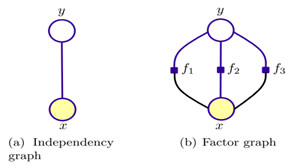
\includegraphics[width=12cm]{0.png}
\caption{两种图模型}
\end{figure}

\begin{equation}
	Z_{\bar(\lambda)}(x) = \sum\limits_{y \in Y} \prod\limits^{m}_{i=1}exp(\lambda_i f_i(x,y))
\end{equation}

\subsection{最大熵马尔可夫模型}

最大熵模型是在已知经验分布的基础上求解有关特征函数$f(x,y)$的最优的$P(y|x)$概率分布,但它的随机变量y有相互独立的假设,所以不能很好 的描述$y_i, x_i$与$y_{i-1}$的关系,而HMM又有观测独立性假设不能自由的选择特征,所以我们希望找到一个能同时服从马尔可夫性假设和服从最大熵假设的模型解决序列标注的问题。

\subsubsection{对比隐马尔可夫模型(HMM)} 

\begin{equation}
	P(X) = \sum\limits_{y} \prod\limits_{i=1}^{T} p(y_i|y_{i-1})p(x_i|y_i)
\end{equation}

状态序列Y,观测序列X,两个状态转移概率:从$y_{i-1}$到$y_i$的条件概率分布,状态$y_i$的输出观测概率,初始概率。隐马尔可夫模型依赖于已知数据的概率分布,已经历史经验来决定现实决策,但实际能提供训练的数据是少量且稀疏的,我们不能枚举所有的数据分布状况,所以需要在数据稀疏的条件下估计未知$x,y$的条件概率。 

\subsubsection{最大熵马尔可夫模型(MEMM)} 

\begin{equation}
	P_{y_i-1}(y_i|x_i)	= \frac{1}{Z_{\bar(\lambda)}(x_i,Y_{i-1})}exp\left( \sum\limits^{m}_{a}\lambda_a f_a(x_i,y_i) \right), \quad i = 1,2,\cdots,T
\end{equation}

用分布来替代HMM中的两个条件概率分布,它表示从先前状态,在观测值下得到当前状态的概率,即根据前一状态和当前观测预测当前状态。每个这样的分布函数都是一个服从最大熵的指数模型。 

\begin{figure}[!htp]
\centering
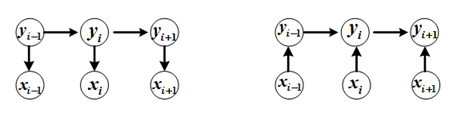
\includegraphics[width=\textwidth]{1.png}
\caption{左为HMM模型,右为MEMM模型}
\label{左为HMM模型,右为MEMM模型}
\end{figure}

\subsubsection{总结} 

HMM:双状态转移条件概率的输出独立性假设,在训练过程通过统计的联合概率,在解码中通过联合概率反向递推的条件概率。

MEMM:限定条件求最优条件概率分布,在训练过程中收敛一组有关特征函数的参数向量,以及有关与的正则化因子,在解码过程中直接求得条件概率。 

最大熵马尔科夫模型\upcite{bib:1}把HMM模型和Maximum-Entropy模型\upcite{bib:2} 的优点集合成一个产生式模型(如图(\ref{左为HMM模型,右为MEMM模型})所示),这个模型允许状态转移概率依赖于序列中彼此之间非独立的特征上,从而将上下文信息引入到模型的学习和识别过程中,提高了识别的精确度,召回率也大大的提高。

\section{问题一模型建立与求解}
为了建立数学模型,找出每个律师擅长的某个或几个专业领域,并对律师回复水平及专业水准进行评估,并用实例验证模型,我们进行了以下工作:

\begin{enumerate}
	\item 将每一篇回复历史进行分词和词频统计。
	\item 综合所有回复,人工挑选出最能代表六个专业领域且词频较高的关键词。
	\item 分别将这些关键词与3000份律师的回复进行匹配,别分统计六个专业领域出现词频最高的前50\%的回复文档,将它们对应的律师判定为擅长该专业领域。
	\item 检索在某个领域排名靠前的若干位律师的文档,阅读他的回复,进行判断来验证模型。
\end{enumerate}

\subsection{词频统计}
在词频统计中,我们首先通过Python中分词开源库搜索引擎模式完成材料的词汇划分与提取。再通过C++编制了一套仿照Python中nltk包的词频特性统计程序完成词频的统计分析与无效字符剔除。

为了降低人工筛选特征词的工作强度,我们首先对3000份文档进行随机抽样,从3000个律师的材料中随机抽取100份文档进行词频分析,我们认为这100份文档产生的所有词可以代表3000份文档产生的大部分词语。我们的部分文档的词频分析结果如图(\ref{部分分词统计结果})所示:

\begin{figure}[!htp]
\centering
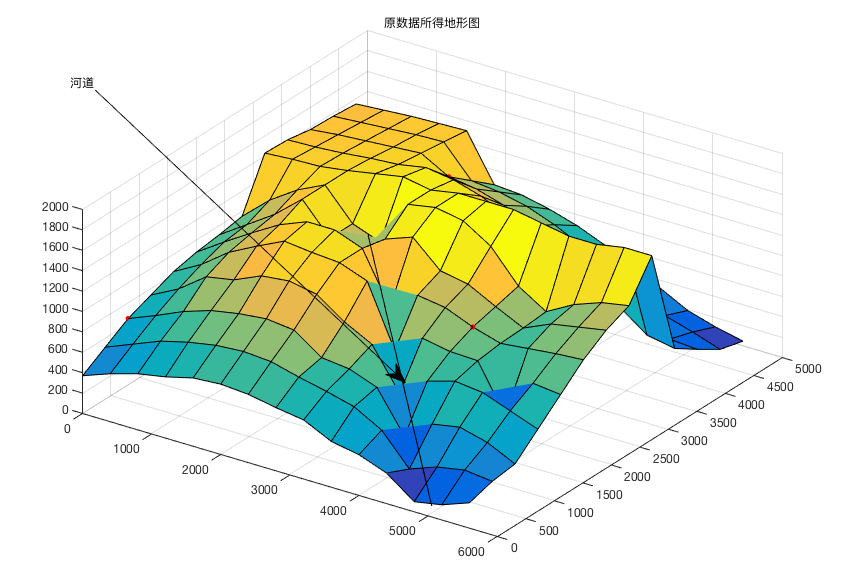
\includegraphics[width=\textwidth]{2.png}
\caption{部分分词统计结果}
\label{部分分词统计结果}
\end{figure}

\subsection{人工筛选}
对于已经统计出每个词的频率,可见像诸如“你好”,“法律”等这些词虽然出现的频率极高,但是并不具有本文中六大法律领域的代表意义,因此我们需要明确我们的选词标准,我们对词语的选择标准是:具有明显法律背景,且仅在某一法律领域具有代表性。为提高我们选词的精度,人工筛选分为两次进行。

初步筛选:阅读100份词频统计结果,将符合上述结果的词添加至法律子项目,结果如图(\ref{初步筛选结果})所示:

\begin{figure}[!htp]
\centering
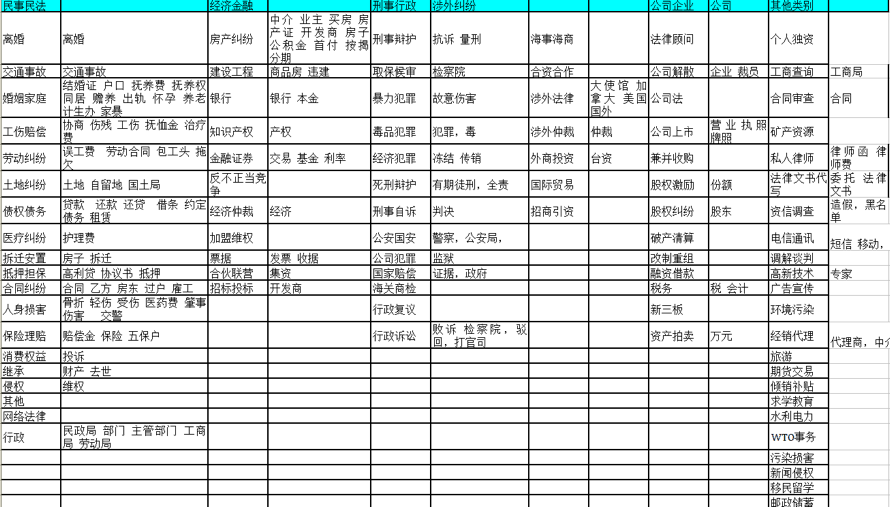
\includegraphics[width=\textwidth]{3.png}
\caption{初步筛选结果}
\label{初步筛选结果}
\end{figure}

精细筛选:每一大的法律领域筛选出十个最具代表性的词或者字用来做为这一领域的特征词,比如像是“受伤”“打伤” “受伤”这类词,我们用 “伤”这一个字来代表这一类民事民法,这样做可以降低检索所需时长。按这样的方法,我们每个法律领域选出10个词代表该法律领域,选出的结果,如表(\ref{关键词筛选结果})所示:

\begin{table}[!htp]
\center
\caption{关键词筛选结果}
\label{关键词筛选结果}
    \begin{tabular}{|l|l|l|l|l|l|l|l|l|l|l|}
    \hline
    民事民法 & 婚  & 交通  & 车  & 同居 & 出轨  & 疗  & 假  & 贷  & 借  & 拆   \\ \hline
    经济金融 & 房  & 公积金 & 首付 & 分期 & 产权  & 交易 & 基金 & 利率 & 发票 & 集资  \\ \hline
    刑事行政 & 刑  & 政   & 贿  & 判  & 狱   & 公安 & 局  & 委  & 暴  & 犯   \\ \hline
    涉外纠纷 & 仲裁 & 台资  & 贸易 & 美国 & 大使  & 国外 & 合资 & 外资 & 海  & 加拿大 \\ \hline
    公司企业 & 公司 & 企   & 股  & 收购 & 税   & 万元 & 资产 & 份额 & 执照 & 裁员  \\ \hline
    其他类别 & 函  & 文书  & 委托 & 短信 & 移动  & 联通 & 电信 & 广告 & 环境 & 代理  \\ \hline
    \end{tabular}
\end{table}

\subsection{匹配选出律师擅长的领域}
\subsubsection{标准建立}
我们已经选出代表每个领域的特征词,我们在对每个律师匹配之前,我们需要对擅长的领域建立一个标准。每个律师在选择他要回答的问题的时候就已经表明他在这六个领域所擅长的某一个领域或某几个领域,我们用每个律师在每个领域回答问题的数量做为律师在这几个领域的评分,通过将每一领域这3000名律师的评分选取前1500名的律师,我们认为这样的律师是擅长这一领域的。例如在民事民法这一领域,排名前1500名的律师我们认为,该律师擅长民事民法。

\subsubsection{算法分析}
该算法的思想是用已经选出的6个法律领域的60个词去匹配问题。具体算法是,首先先对这3000个律师中的所有问题用民事民法中的10个特征词进行筛选,只要出现十个词中的一个即在民事民法中记一分,并直接对下一个问题进行同样地分析,当分析完所有的民事民法,得到该律师在民事民法的得分。接下来对下一个律师进行同样的民事民法分析,做完3000个律师的民事民法分析,通过3000个律师得分的前1500名,我们认为这1500个律师是擅长这一领域的。同理对于其他领域可以进行同样地分析。表(\ref{各领域律师排名(前五)})给出每个领域排名前五的律师作为示例。

\begin{table}[!htp]
\center
\caption{各领域律师排名(前五)}
\label{各领域律师排名(前五)}
    \begin{tabular}{|c|c|c|c|c|c|c|c|c|}
    \hline
    民事民法 & 编号   & 相关回答 & 经济金融 & 编号   & 相关回答 & 刑事行政 & 编号   & 相关回答 \\ \hline
    1    & 2899 & 383   & 1    & 1142 & 349   & 1    & 2315 & 389   \\ \hline
    2    & 2583 & 377   & 2    & 1287 & 315   & 2    & 998  & 379   \\ \hline
    3    & 893  & 342   & 3    & 497  & 295   & 3    & 538  & 369   \\ \hline
    4    & 809  & 341   & 4    & 647  & 290   & 4    & 1485 & 366   \\ \hline
    5    & 845  & 341   & 5    & 2711 & 275   & 5    & 180  & 360   \\ \hline
    涉外纠纷 & 编号   & 相关回答 & 公司企业 & 编号   & 相关回答 & 其他类别 & 编号   & 相关回答 \\ \hline
    1    & 2839 & 118   & 1    & 2583 & 325   & 1    & 2315 & 384   \\ \hline
    2    & 1798 & 103   & 2    & 2839 & 240   & 2    & 998  & 374   \\ \hline
    3    & 2373 & 102   & 3    & 2063 & 222   & 3    & 538  & 357   \\ \hline
    4    & 353  & 96    & 4    & 1245 & 185   & 4    & 162  & 341   \\ \hline
    5    & 1390 & 96    & 5    & 805  & 178   & 5    & 13   & 340   \\ \hline
    \end{tabular}
\end{table}

并对最擅长各个领域的律师研究了他们其他擅长的方向,如表(\ref{各领域排名第一的律师的领域分析})所示:(表中1代表擅长,0代表不擅长)。

\begin{table}[!htp]
\center
\caption{各领域排名第一的律师的领域分析}
\label{各领域排名第一的律师的领域分析}
    \begin{tabular}{|c|c|c|c|c|c|c|}
    \hline
    编号   & 民事民法 & 经济金融 & 刑事行政 & 涉外纠纷 & 公司企业 & 其他类别 \\ \hline
    2899 & 1    & 0    & 0    & 0    & 0    & 0    \\ \hline
    2583 & 1    & 1    & 1    & 1    & 0    & 0    \\ \hline
    2315 & 1    & 0    & 1    & 0    & 1    & 0    \\ \hline
    2839 & 0    & 1    & 0    & 1    & 1    & 1    \\ \hline
    2583 & 1    & 1    & 1    & 1    & 0    & 0    \\ \hline
    2315 & 1    & 0    & 1    & 0    & 1    & 0    \\ \hline
    \end{tabular}
\end{table}

\subsection{对律师的回复水平进行评价}
\subsubsection{标准建立}
在评价律师的回答问题的好坏时评价的标准仅从回答的长度来判断。我们选取这样的评价标准并没有具体考虑到回答的专业性,回答的详细程度,回答的严谨程度,我们认为在这样的一个律师回答平台,每个律师回答的字数越多往往可以代表着,回答的比较专业,回答的详细,回答的比较严谨。另外我们不容易将这些专业性,严谨性,详细度这些指标无法在机器学习中得以很好的刻画。
\subsubsection{算法分析}

通过对每个律师回答的字数统计,按照由高到低的顺序排序,排序越靠前的则表明该律师的回复水平越高。

\subsubsection{结果检验}

\subsubsection*{对法律领域擅长方向的检验}

首先每个律师回答问题均为400道,同时根据关键词筛选分类问答的总数小于400个,说明我们筛的关键词比较明确无歧义,一般不造成领域间的混淆,并且通过阅读文档实际找寻对律师的回复领域的检验发现律师确实对于该方面的回答很多。例如2899号律师的确主要解决民事问题。

我们认为只要排名在在前1500即可认为擅长这一领域,则每个律师平均擅长的领域有3个。

\begin{table}[!htp]
\center
\caption{律师的擅长领域分析}
\label{律师的擅长领域分析}
    \begin{tabular}{|c|c|c|c|c|c|c|}
    \hline
    擅长0个   & 擅长1个 & 擅长2个 & 擅长3个 & 擅长4个 & 擅长5个 & 擅长6个 \\ \hline
    60 & 325    & 672   & 887    & 684    & 300    & 72    \\ \hline

    \end{tabular}
\end{table}

擅长不同类别不同数量的人数呈现正态分布,说明我们用排名1500名作为分界线是较为合理的。

\subsubsection*{对律师的而回答质量和水平检验}

通过排序我们发现平均回复长度前5名(括号内为平均回复字数)是652号律师(516),776号律师(774), 58号律师(294), 2114号律师(232), 436号律师(226) 。最后5名是1300号律师(10), 1043号律师(9), 1218号律师(9), 2163号律师(8), 328号律师(7)。

注:通过我们实际查阅652号律师的问答,发现大部分的回答都是很长相同的话,故舍弃不用,选取排名第二的776号律师进行分析。

下面我们截取776号律师和328号律师的回答进行截取验证,验证如下:


\begin{figure}[!htp]
\centering
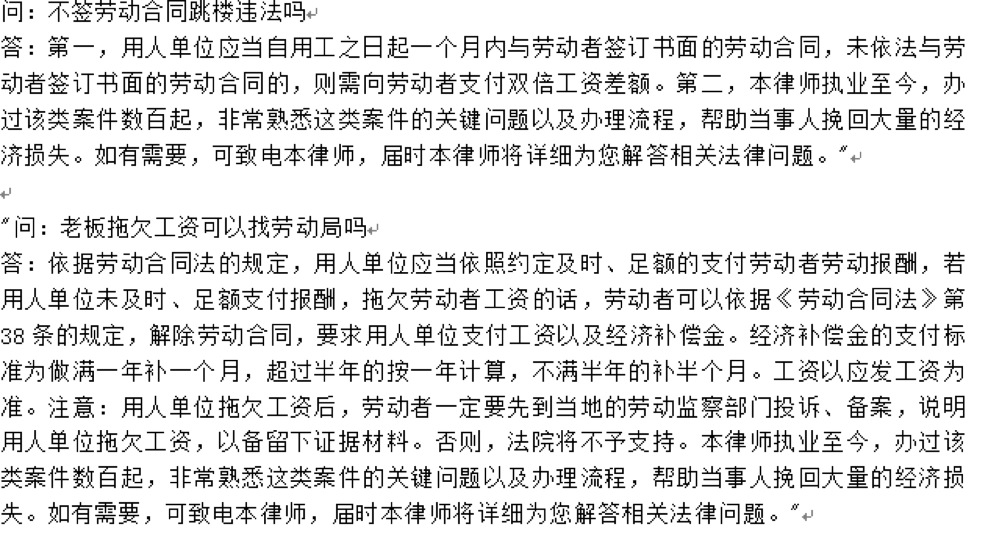
\includegraphics[width=12cm]{4.png}
\caption{776号律师回答摘要}
\label{776号律师回答摘要}
\end{figure}


\begin{figure}[!htp]
\centering
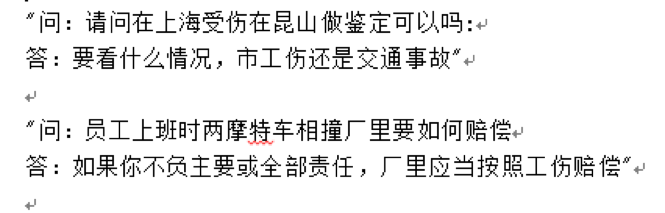
\includegraphics[width=10cm]{5.png}
\caption{328号律师回答摘要}
\label{328号律师回答摘要}
\end{figure}

由图(\ref{776号律师回答摘要},\ref{328号律师回答摘要})可见,776号律师的回答要比328号律师详尽很多,且严谨很多,并且说话有依据,以及思考的方面也比328号全面的多

\section{问题二模型建立与求解}

在问题1中,我们已经有了两个指标:第一个是通过分别将这些关键词与3000份律师的回复进行匹配,统计六个专业领域出现词频最高的前50\%的回复文档,将它们对应的律师判定为擅长该专业领域。这个排序我们已知。第二个是我们已分别统计3000份回复中律师回答字数的平均值,排序我们也已知道。因而我们将这两个指标的平均作为我们推荐律师的判定综合指标,分数确定如下:

\begin{enumerate}
	\item 3000位律师中,六个专业领域出现词频最高的得3000分,第二名得2999分,依次递减。
	\item 3000位律师中,回答字数的平均值最高的得3000分,第二名得2999分,依次递减。
	\item 3000位律师在各个专业的指标为他在该专业出现词频得分与回答字数的平均值得分的平均。
\end{enumerate}

通过这样一个综合指标,我们既考虑了律师回答某领域的问题数也考虑了他回答的水平。

综合指标排序结果如表(\ref{各领域综合比指标排名})所示:(截取的各领域前10)

\begin{table}[!htp]
\center
\caption{各领域综合比指标排名}
\label{各领域综合比指标排名}
    \begin{tabular}{|c|c|c|c|c|c|c|}
    \hline
    编号   & 民事民法 & 经济金融 & 刑事行政 & 涉外纠纷 & 公司企业 & 其他类别 \\ \hline
    2899 & 1    & 0    & 0    & 0    & 0    & 0    \\ \hline
    2583 & 1    & 1    & 1    & 1    & 0    & 0    \\ \hline
    2315 & 1    & 0    & 1    & 0    & 1    & 0    \\ \hline
    2839 & 0    & 1    & 0    & 1    & 1    & 1    \\ \hline
    2583 & 1    & 1    & 1    & 1    & 0    & 0    \\ \hline
    2315 & 1    & 0    & 1    & 0    & 1    & 0    \\ \hline
    \end{tabular}
\end{table}

指标确定后,我们按照以下的步骤处理:

\begin{enumerate}
	\item 在客户输入的案情描述搜索我们在六个专业领域中挑选出的关键词,从而确定案情属于的专业领域。
	\item 挑选若干位在该领域总指标靠前的律师。
	\item 手工查阅推荐编号的律师的问答记录,验证模型。
\end{enumerate}

\subsection{关键词提取}

关键词提取与问题一类似,不同之处在于在对该客户输入案情描述的匹配过程中,可能出现大于一个领域的特征词语。因而可能推荐大于一个领域的律师。这也与实际生活是吻合的,有些案情可能涉及多个专业领域。

\subsection{分配律师}

关键词提取并匹配过后,我们就确定了这一案情涉及的领域。而我们也已经分别得到了六个领域律师综合指标的排序。根据用户需要的推荐律师的数目,只需按所需数量取出即可。

\subsection{结果检验}

\subsubsection*{综合指标的合理性检验}


以民事民法综合指标排名第一的1179号律师为例,他在民事民法方面的回答均很完善。对于问题的回答不仅有针对性,而且基于事实,也基于法律。不管是分类说明还是阐述,他的回答均非常完整且清晰。如图(\ref{1179号律师回答摘要1},\ref{1179号律师回答摘要2})所示两个问答例子:

\begin{figure}[!htp]
\centering
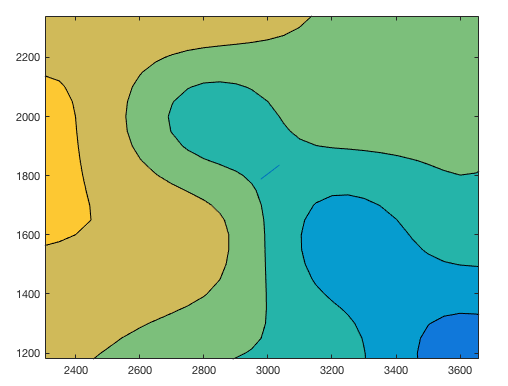
\includegraphics[width=\textwidth]{6.png}
\caption{1179号律师回答摘要1}
\label{1179号律师回答摘要1}
\end{figure}

\begin{figure}[!htp]
\centering
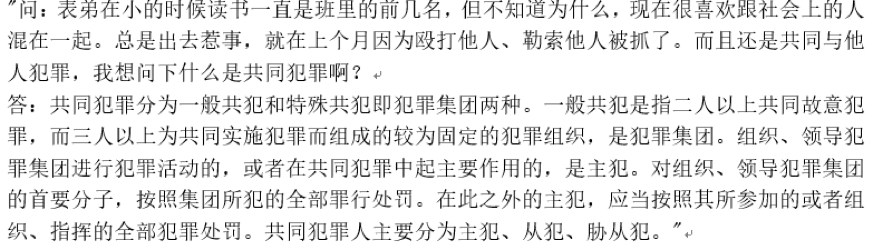
\includegraphics[width=\textwidth]{7.png}
\caption{1179号律师回答摘要2}
\label{1179号律师回答摘要2}
\end{figure}


如图(\ref{1928号律师回答摘要})经济金融领域综合指标排名第一的1928号律师,也条理清晰、有理有据。

\begin{figure}[!htp]
\centering
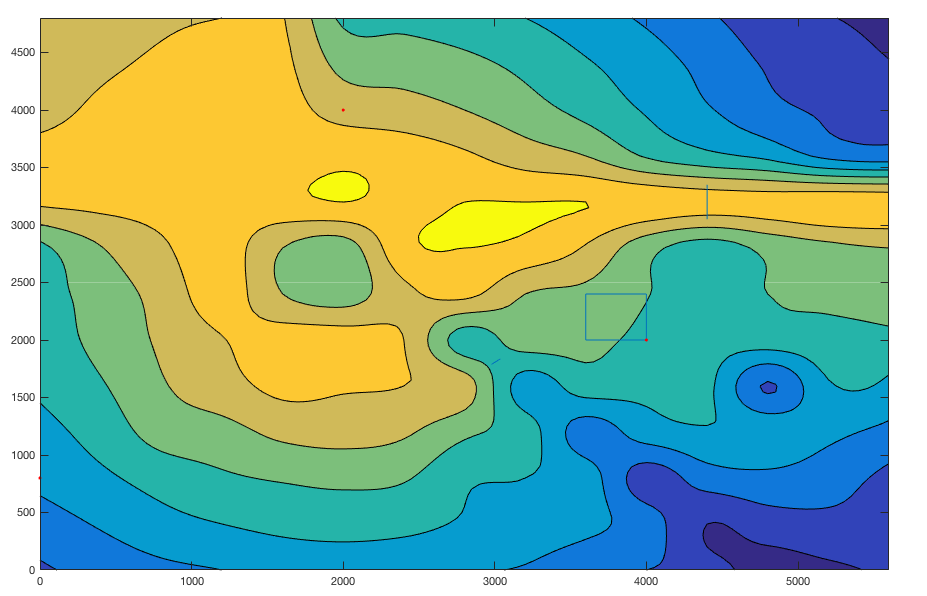
\includegraphics[width=\textwidth]{8.png}
\caption{1928号律师回答摘要}
\label{1928号律师回答摘要}
\end{figure}

相反,查看涉外纠纷领域综合指标最后一名的1043号律师(如图(\ref{1043号律师回答摘要})所示),得分19。在其回答中仅出现“咨询”二字,没有任何有效信息。说明我们综合了回复题目数量和回复字数的综合指标行之有效。

\begin{figure}[!htp]
\centering
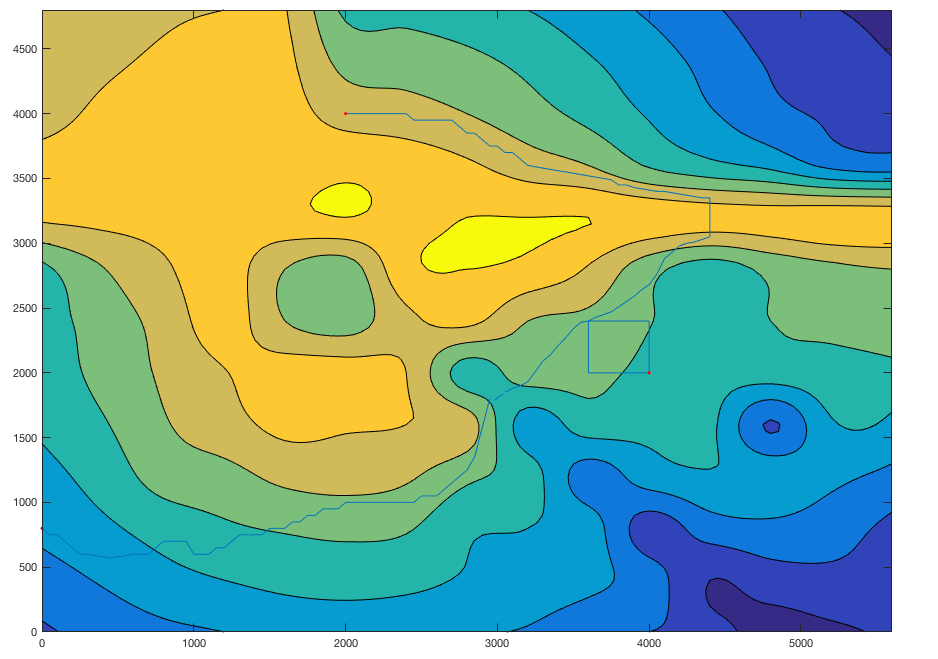
\includegraphics[width=\textwidth]{9.png}
\caption{1043号律师回答摘要}
\label{1043号律师回答摘要}
\end{figure}

\subsubsection*{推荐律师检验}

我们尝试向律师推荐程序键入问题,该问题中涉及到的特征词有房、拆,因而跟民事民法和经济金融有直接关联。程序运行后按照预期推荐了两大类共计6位律师,如图(\ref{律师推荐程序实验})所示。

\begin{figure}[!htp]
\centering
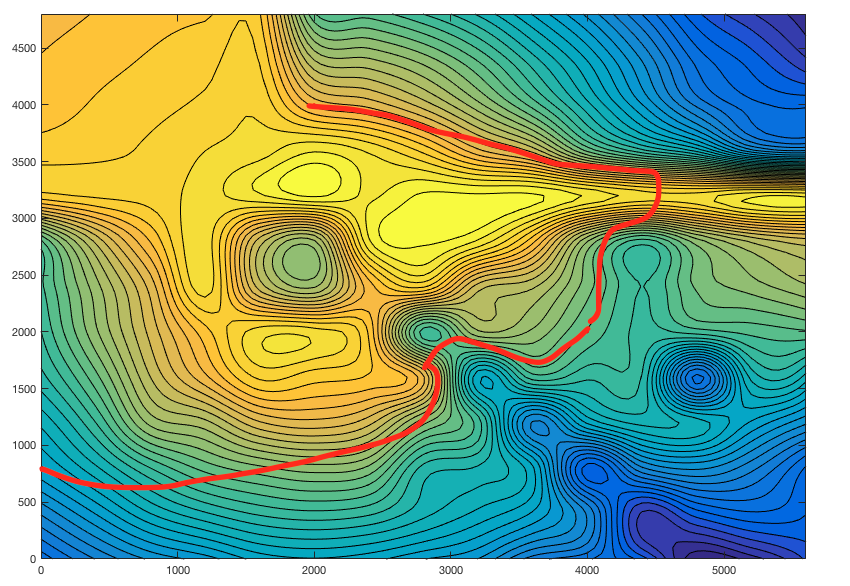
\includegraphics[width=\textwidth]{10.png}
\caption{律师推荐程序实验}
\label{律师推荐程序实验}
\end{figure}


例如检索2583号律师的文档发现,其针对这方面问题的回答较为优质,基本验证我们律师推荐算法的可行性。

\section{问题三模型建立与求解}
\subsection{方法与思路}
\subsubsection*{方法1}

在客户输入的案情描述搜索我们在六个专业领域中挑选出的关键词,从而确定案情属于的专业领域。挑选若干位在该领域排名靠前的律师,在他们的回复中通过匹配关键词进行查找,选出最贴近的回答进行显示。

\subsubsection*{方法2}

根据客户输入的案情描述,通过爬虫登录搜索引擎,将访问量最高的回复返回给客户。

\subsection{结果检验}

本题中我们采用方法1进行验证。但由于我们是用匹配特征词语进行查找的,因而如果问题不带有特征词语的时候算法会失效。我们随机验证了两个情况,如图(\ref{自动回答程序实验})所示。

\begin{figure}[!htp]
\centering
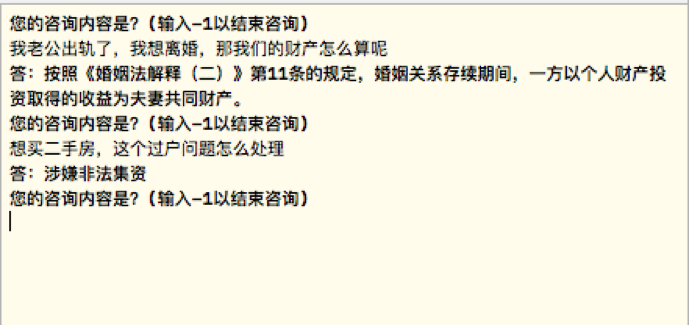
\includegraphics[width=10cm]{11.png}
\caption{自动回答程序实验}
\label{自动回答程序实验}
\end{figure}

第一个情况,非常的贴切,通过婚以及出轨都能定位出这是民事民法领域,再在推荐律师的文档中进行问题特征词语的匹配,最终得到答案,效果挺好。

但第二个情况,通过房定位到经济金融,但可能含有特征词语只有一个,因而得到了不理想的结果。暴露了该算法需要用户提出的问题中尽可能多地包含特征词语且过度依赖已有回答的弊端。


\section{模型的优缺点}

\subsection{优点}
\begin{enumerate}
	\item 在选择律师擅长的方面时,用律师在某一领域回答问题的数量在3000个律师中的排名来做到,更具有客观性。
	\item 在评价律师评价水平时选择用律师回答的长度来评价,思路简明,认为在一个律师专业咨询平台的回答,往往越长,即代表着回答的更加详细,更专业,更加严谨。这样便省去对多因素分配权重。
	\item 在推荐律师时,考虑了出现不同专业领域关键词的情况,符合实际。现实中问题可能会涉及到大于一个专业领域。
	\item 利用机器学习进行分词,再人工结合专业领域进行筛选,选出的词兼具概括性和高词频的特点。
\end{enumerate}

\subsection{缺点}

\begin{enumerate}
	\item 在找寻律师的擅长领域,按照我们的寻找标准,单个律师的回答特定领域问题数在所有3000个律师中的排名在前1500名认为擅长,有可能会存在一些律师没有擅长的领域存在,或者极个别律师擅长所有领域的情况。
	\item 在找寻律师的擅长领域,我们用单个律师的回答特定领域问题数在所有3000个律师中的排名这一标准的一个前提假设是每个律师回答的总问题数是相同的,更精确可以将数量排名换成比例。
	\item 在评价律师的回答问题的好坏时评价的标准仅从回答的长度来判断,没有证明回答的详细程度与专业性,严谨性有明显的正向相关关系。
	\item 问题3中由于我们是用匹配特征词语进行查找的,因而如果问题所有特征词语一个都不带有的时候算法会失效。
\end{enumerate}

\section{模型改进方向}
\begin{enumerate}
	\item 在第二文中我们推选适合的律师的时候我们只是考虑律师在第一问中的的擅长程度,即,律师回答某专业的问题的多少在全体律师中的排名,我们会选取排名靠前的若干律师推送给客户,但是并没有具体考虑律师回答问题的详细程度,即没有考虑律师回答专业水平这一指标,因此我们在模型改进中应该综合上述的这两个指标。
	\item 如果需要提高精度,就需要考虑本文6大法律领域的子法律,分类细化,找到更适合的律师,做到更高效率。
\end{enumerate}
\begin{thebibliography}{9}
 \bibitem{bib:1} \url{http://wiki.swarma.net/index.php/}
 \bibitem{bib:1} \url{http://blog.sina.com.cn/s/blog_8af106960102v0v1.html}
\end{thebibliography}
\appendix

\section{}
\section*{程序源码}

分词处理\textcolor[rgb]{0.98,0.00,0.00}{\textbf{Input Python source:}}
\lstinputlisting[language=Python]{./code/分词处理.py}
模仿NLTK进行关键词筛选与统计\textcolor[rgb]{0.98,0.00,0.00}{\textbf{Input C++ source:}}
\lstinputlisting[language=C++]{./code/关键词匹配统计.cpp}
第一问:按照回答长度划分律师回答水平\textcolor[rgb]{0.98,0.00,0.00}{\textbf{Input C++ source:}}
\lstinputlisting[language=C++]{./code/按回答长度律师专业程度处理.cpp}
第二问:综合领域分类关键词匹配度排序以及回答长度的综合指标处理\textcolor[rgb]{0.98,0.00,0.00}{\textbf{Input C++ source:}}
\lstinputlisting[language=C++]{./code/综合回答按类别排名.cpp}
第二问:律师选择推荐程序\textcolor[rgb]{0.98,0.00,0.00}{\textbf{Input C++ source:}}
\lstinputlisting[language=C++]{./code/第二问选择律师.cpp}
第三问:自动回答系统的尝试\textcolor[rgb]{0.98,0.00,0.00}{\textbf{Input C++ source:}}
\lstinputlisting[language=C++]{./code/自动回答系统尝试.cpp}



\end{document} 